




\section{MEASUREMENT SETUP} \label{sec:exp setup}

Experiments were performed on a QPU comprising 11 uncoupled superconducting qubits hosted in a dilution refrigerator. Control and readout were implemented using a Quantum Machines OPX platform together with microwave components from Keysight Technologies, including IQ mixers, local oscillators (LOs), attenuators, filters, and amplifiers.

A schematic of the setup is shown in Fig.~\ref{fig:diagram}. At room temperature, baseband I/Q waveforms are generated by arbitrary waveform generators (AWGs) and upconverted to microwave frequencies using IQ mixers driven by LOs. Separate lines are used for qubit drive and resonator readout. In addition, a dedicated DC bias line provides static flux control.

The microwave signals are routed into the dilution refrigerator through heavily attenuated and filtered coaxial lines. Attenuators are distributed across multiple temperature stages (300 K to $\sim$9 mK) to thermalize the lines and suppress room-temperature noise. Additional filtering (low-pass and infrared filters) further reduces high-frequency noise before the signals reach the device.

The quantum device is mounted at the mixing chamber stage ($\sim$9 mK). The outgoing readout signal is routed through a chain of circulators that isolate the qubit from amplifier back-action, followed by cryogenic amplification using a high-electron-mobility transistor (HEMT) amplifier at the 4 K stage. The signal is then further amplified, downconverted, and digitized at room temperature.

Digitized signals are processed in real time and used for classical post-processing and iterative experiment execution.


\begin{figure}
    \centering
    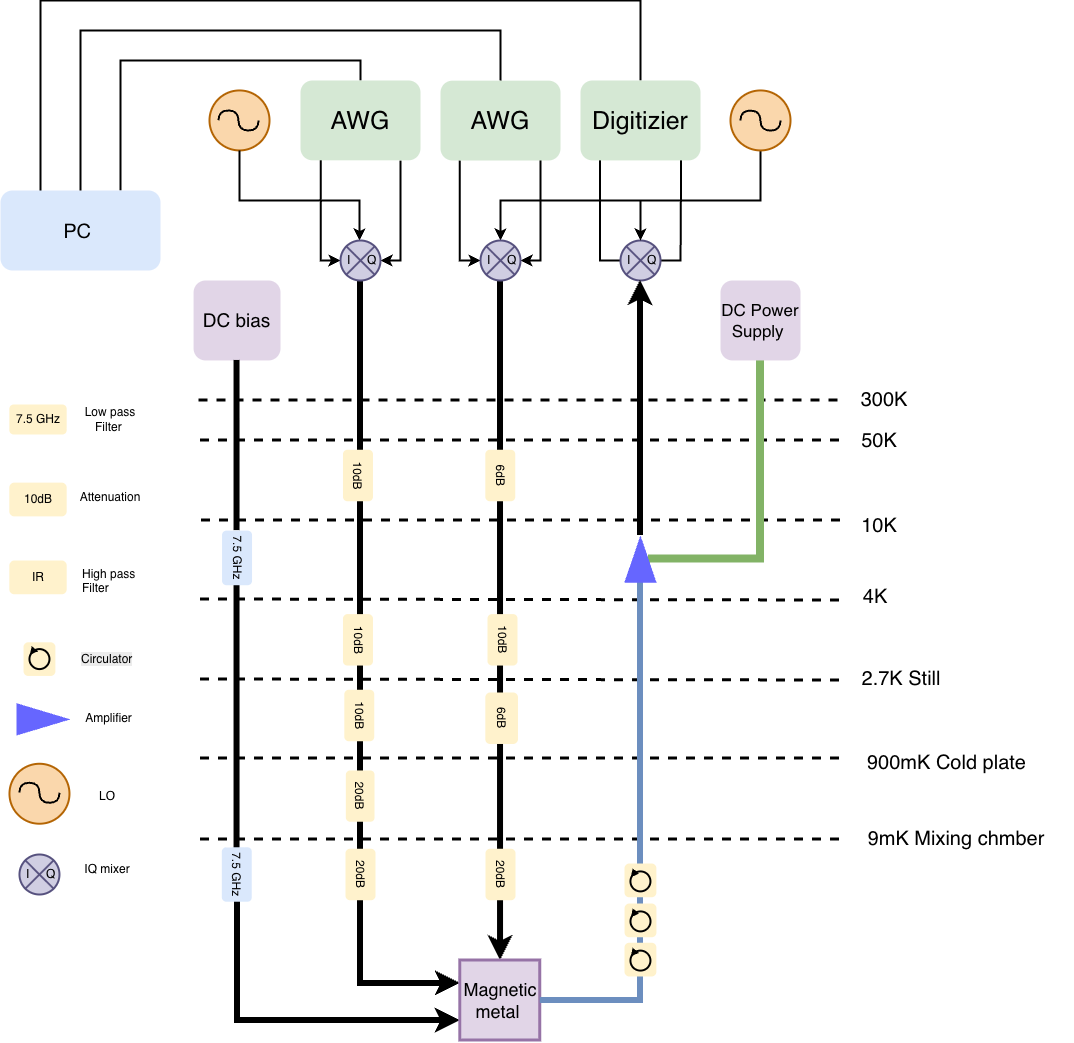
\includegraphics[width=1\linewidth]{figures/diagram_v2.drawio (1).png}
    \caption{Schematic of the experimental setup for qubit control and readout.
Room-temperature electronics (top) include a computer controlling two arbitrary waveform generators (AWGs) and a digitizer. The AWGs generate baseband I/Q signals that are upconverted to microwave frequencies via IQ mixers driven by local oscillators (LOs), enabling qubit drive and resonator readout. The signals are routed into a dilution refrigerator (dashed region), where multiple temperature stages (38 K, 10 K, 2.7 K, 900 mK, and 9 mK) are indicated. Input lines are attenuated and filtered at each stage to suppress thermal noise before reaching the device. The output signal is routed through circulators and amplified by a cryogenic high-electron-mobility transistor (HEMT) amplifier before being further processed at room temperature and digitized. The quantum device is mounted at the base temperature stage (~9 mK). }
    \label{fig:diagram}
\end{figure}

\section{$T_2$ limit} \label{sec:T2_limit}

The Bloch equations \cite{PhysRev.70.460} provide a theoretical framework for describing the dynamics of a two-level system under an external excitation field with strength $\Omega_0$, frequency detuned from natural qubit frequency with detuning $\Delta,$ including presence of  relaxation and dephasing times $T_1$ and $T_2$. Originally developed in the context of NMR, the Bloch equations are equally applicable to superconducting qubits.

The formalism is based on solving a system of differential equations for the expectation values of the qubit's Pauli operators, $\sigma_x$, $\sigma_z$ and $\sigma_z$ , which together give full information of the qubit state. 

A key advantage of the Bloch solution is its validity across a broad range of excitation pulse durations, from short to long, and for both weak and strong driving fields (however, to prevent leakage into higher energy levels, the drive amplitude must remain below the qubit’s anharmonicity).

In our study, we focus on the regime where the solution to the Bloch equations describes long-duration pulses, such that the qubit undergoes complete energy saturation $t\gg T_1$. In this limit, for resonance pulses, the qubit reaches a mixed state, and its evolution is a simple closed-form solution. In particular, we are interested in the expectation value $\left<\sigma_z\right>$, which serves as the measurable observable of our system:
\begin{equation}
\left<\sigma_z\right> =\frac{1+(T_2\Delta)^2}{1+(T_2\Delta)^2+\Omega_0^2T_1T_2}
\label{eq:bloch_solution}
.\end{equation}
The solution determines the linewidth at broad range of cases and will be applicable to understand the limits for high resolution spectroscopy.

\subsection{Linewidths and Saturation Spectroscopy}

In the strong-driving regime, where the Rabi frequency dominates the detuning term,
\[
\Omega_0 \gg \sqrt{\frac{T_2}{T_1}}\,\Delta,
\]
Eq.~(\ref{eq:bloch_solution}) simplifies to
\begin{equation}
    \langle \sigma_z \rangle
    \approx
    1 - 2\frac{1}{1 + \dfrac{\Delta^2}{(T_1/T_2)\Omega_0^2}}.
\end{equation}
In this limit, the transition linewidth is broadened to
\begin{equation}
    \Delta_{1/2,\Omega_0}
    =
    \frac{2\Omega_0}{\sqrt{T_2/T_1}}.
\end{equation}
This phenomenon, known as \emph{power broadening} (or saturation broadening), is analogous to the linewidth increase observed in Rabi spectroscopy. Here, however, the broadening arises from saturation of the transition and the resulting population redistribution between the qubit states.

In contrast, in the weak-driving regime,
\[
\Omega_0 \ll \sqrt{\frac{T_2}{T_1}}\,\Delta,
\]
the excitation remains far from saturation, and the linewidth is determined solely by the qubit coherence time. In this case, Eq.~(\ref{eq:bloch_solution}) reduces to
\begin{equation}
    \langle \sigma_z \rangle
    \approx
    1
    -
    2\Omega_0^{2}T_1T_2
    \frac{1}{1 + T_2^{2}\Delta^{2}},
\end{equation}
which has a Lorentzian lineshape with a minimum achievable linewidth set by $T_2$:
\begin{equation}
    \Delta_{1/2,T_2}
    =
    \frac{2}{T_2}.
    \label{eq:T2_limit}
\end{equation}
This represents the coherence-limited linewidth of the qubit transition and constitutes the fundamental resolution limit of conventional continuous-wave spectroscopy.




\section{Appendix cutoff} \label{sec:cutoff}

\begin{figure}
    \centering
    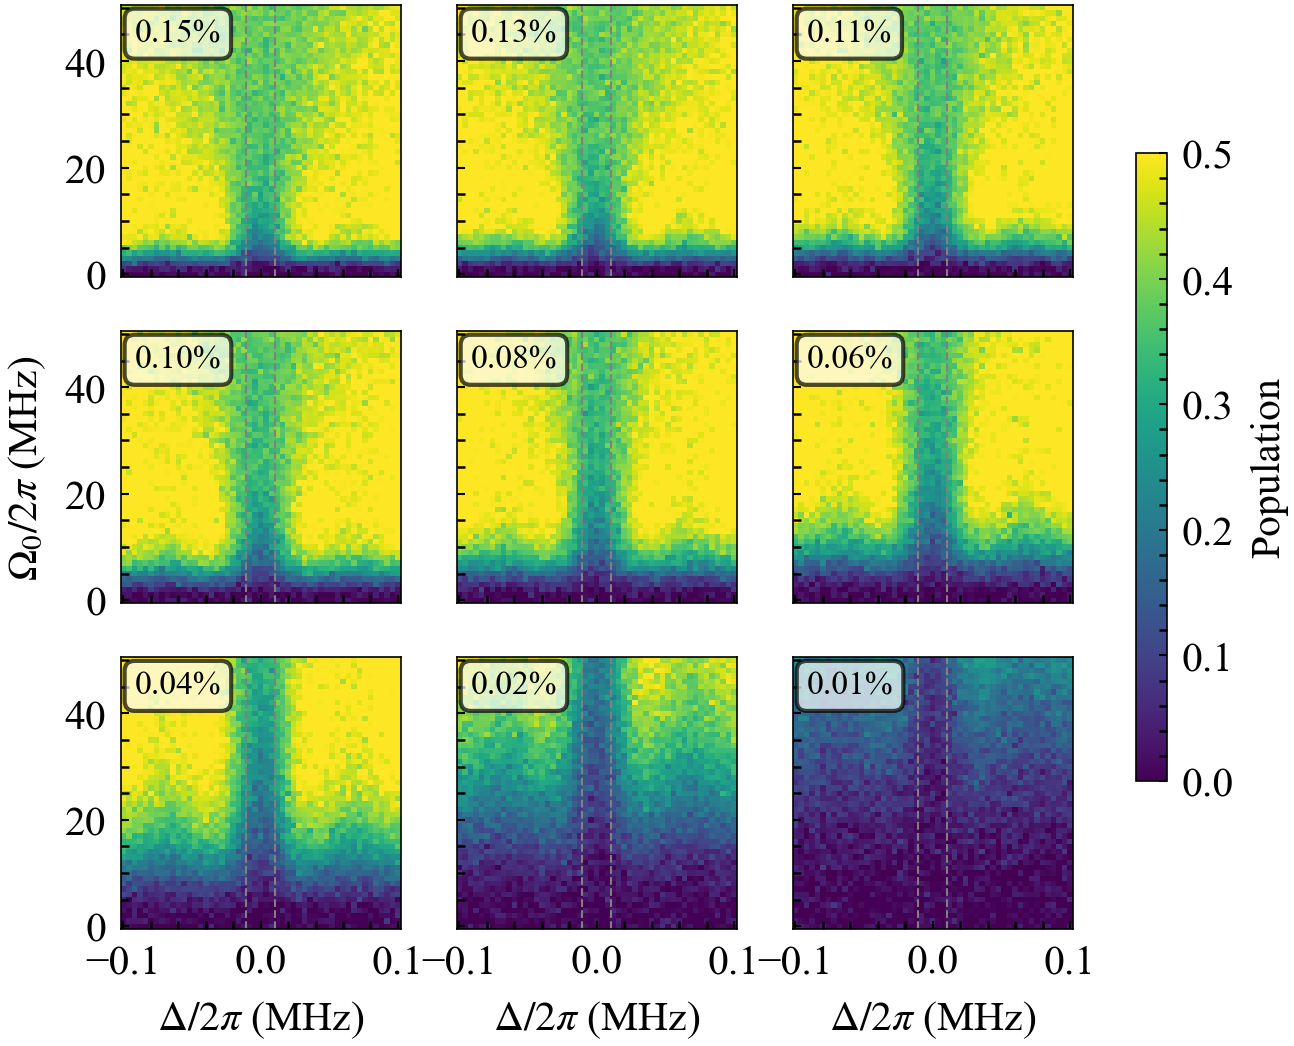
\includegraphics[width=1\linewidth]{figures/spectroscopy_cutoff_comparison.png}
    \caption{Spectroscopic response obtained using echo–root–Lorentzian pulses for different relative cutoff amplitudes (indicated in the upper-left corner of each panel). Increasing the cutoff smooths the phase inversion point of the pulse, thereby suppressing derivative discontinuities that otherwise induce residual power broadening. As a result, the spectral line becomes progressively narrower and more robust to drive-amplitude variations. However, for excessively small cutoff values the effective signal-to-noise ratio deteriorates, limiting the attainable spectral contrast despite reduced broadening.}
    \label{fig:placeholder}
\end{figure}
The spectral linewidths corresponding to the two regimes are given by
\[
\Delta_{1/2,T_2} = \frac{1}{\pi T_2}, \qquad \Delta_{1/2,\Omega_0} = \frac{\Omega_c}{\pi \sqrt{T_2/T_1}}.
\]
Requiring $\Delta_{1/2,T_2} < \Delta_{1/2,\Omega_0}$ yields
\[
\Omega_c < \frac{1}{\sqrt{T_1 T_2}}.
\]
If we express the coupling strength as $\Omega_c = c\,\Omega_0$, the condition becomes
\[
c < \frac{1}{\Omega_0 \sqrt{T_1 T_2}}.
\]
Substituting $T_1 = 30~\mu\text{s}$, $T_2 = 15~\mu\text{s}$, and $\Omega_0 = 50~\text{MHz}$ gives
\[
c < 9.4 \times 10^{-4},
\]



\begin{figure}
    \centering
    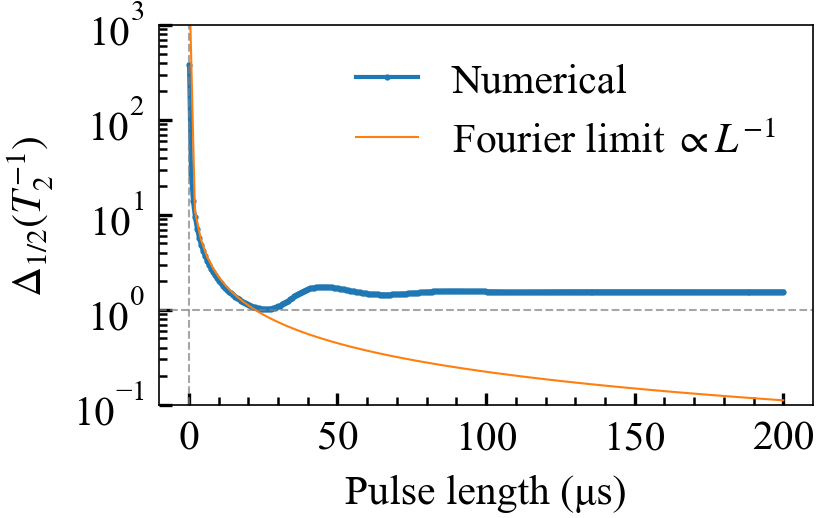
\includegraphics[width=1\linewidth]{figures/length_scan.png}
    \caption{Numerical linewidth $\Delta_{1/2}$
, normalized to the decoherence-limited scale $T_2^{-1}$
, obtained from square-pulse spectroscopy as a function of pulse duration. For short interrogation times, the linewidth decreases inversely with pulse length, following the Fourier limit. For longer pulses, the linewidth saturates at the fundamental $T_2$ limit imposed by decoherence, deviating from the Fourier-limited scaling.}
    \label{fig:fig7}
\end{figure}

\section{Adiabatic Basis} \label{sec:develop}


The matrix form of the Hamiltonian in the rotated frame takes the form:
\begin{equation}
    H(t) = \frac{1}{2}
    \begin{bmatrix}
            -\Delta & \Omega(t) \\ \Omega(t)  & \Delta
    \end{bmatrix}
\label{eq:rotated_hamlitonian_matrix}
.\end{equation}

The Rabi frequency $\Omega(t)$ quantifies the field-induced coupling between the two states. The instantaneous eigenstates of \( H(t) \), commonly referred to as the adiabatic states, are:
\begin{align}
| w_- (t) \rangle &= \cos \vartheta(t) |0\rangle - \sin \vartheta(t) |1\rangle, \\
| w_+ (t) \rangle &= \sin \vartheta(t) |0\rangle + \cos \vartheta(t) |1\rangle
\label{eq:rotating_basis}
,\end{align}
where the mixing angle is given by  $\vartheta(t) = \frac{1}{2}\arctan\frac{\Omega(t)}{\Delta}$. The corresponding eigenvalues, representing the adiabatic energy levels, are:
\begin{equation}
\varepsilon_{\pm}(t) = \frac{\hbar}{2} \left( \Delta \pm \sqrt{\Omega^2(t) + \Delta^2} \right)
,\end{equation}
yielding an energy gap of $\varepsilon(t) =\varepsilon_+(t) - \varepsilon_-(t) = \hbar \sqrt{\Omega^2(t) + \Delta^2}$.

Using the eigenvectors from Eq. (\ref{eq:rotating_basis}) we define the adiabatic transformation matrix $R$. Applying this transformation to the Hamiltonian in Eq. (\ref{eq:rotated_hamlitonian_matrix}) gives the  Hamiltonian in the adiabatic basis $H^{a} = R^{\dagger} H R - i R^{\dagger} \dot{R}$, which can be explicitly written as:



\begin{equation}
    H^a(t) = \frac{1}{2}
    \begin{bmatrix}
            -\varepsilon(t)/2 & -i\dot{\vartheta}(t) \\ \dot{\vartheta}(t)  & \varepsilon(t)/2
    \end{bmatrix}
    .
\end{equation}
Adiabatic evolution requires that the rate of change of the mixing angle \( \vartheta(t) \) is much smaller than the energy splitting $\varepsilon(t)$, leading to the adiabatic condition \cite{adiabatic_theorem,BORADJIEV201391}:
\begin{equation}
| 2\dot{\vartheta}| \ll \varepsilon(t),
\label{eq:adiabtic_condtion}
\end{equation}
where the non-adiabatic coupling term is given explicitly by $| \dot{\vartheta}| = \frac{\Delta\dot{\Omega}(t)}{2[\Delta+\Omega(t)]}$. 



\begin{figure}
    \centering
    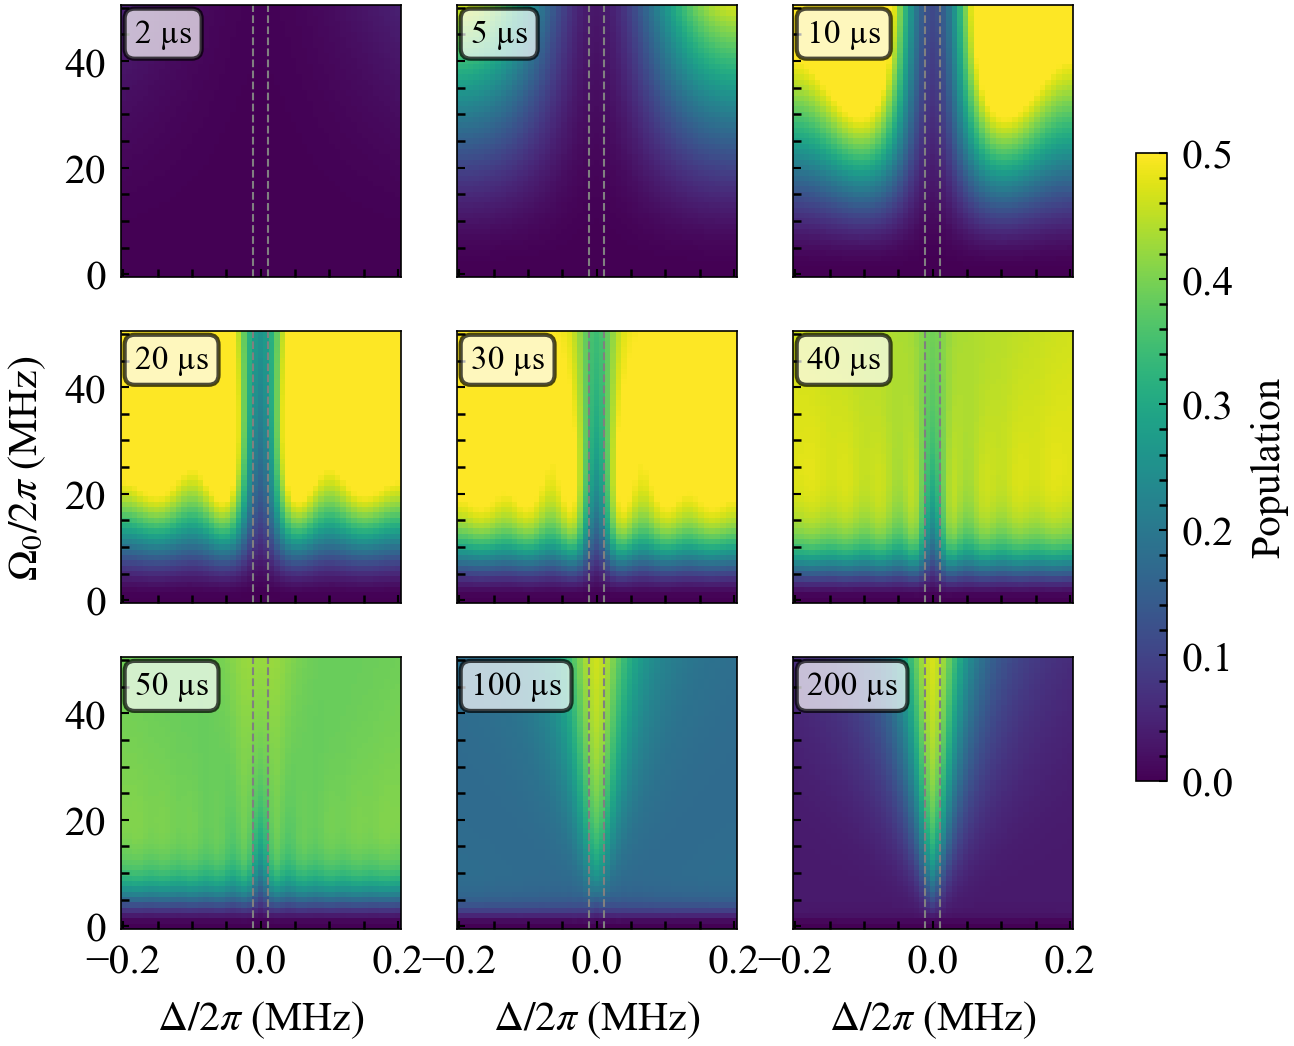
\includegraphics[width=1\linewidth]{figures/spectroscopy_length_comparison.png}
    \caption{Numerical spectroscopic response obtained using echo–root–Lorentzian pulses for different pulse durations (indicated in each panel). As the pulse length increases, the spectral linewidth progressively narrows, approaching the decoherence-limited resolution set by the coherence time $T_2$. For pulse durations comparable to or exceeding the relaxation time $T_1$, population decay during the interrogation leads to an elevated off-resonant background, reducing spectral contrast despite the continued narrowing of the resonance feature.}
    \label{fig:fig8}
\end{figure}




Replacing the inequality in Eq.  (\ref{eq:adiabtic_condtion}) with an equality provides a approximate boundary condition between adiabatic  and non-adiabatic regions
\begin{equation}
   \sqrt{\Omega^2(t_0) + \Delta_b^2}= \frac{\Delta_b\dot{\Omega}(t_0)}{2[\Delta^2+\Omega^2(t_0)]}
,\end{equation}
where $t_0$ denotes the time at which the non-adiabatic coupling $| \dot{\vartheta}|$, is maximal, and  $\Delta_b$  marks the boundary between the adiabatic and non-adiabatic regimes. This condition allows us to extract a threshold value for the detuning range $\Delta<\Delta_b$ which marks the range of detunings where post-pulse excitation remains significant. The excitational linewidth scales proportionally to the threshold detuning  $\text{FWHM}\propto\Delta_b$. Consequently, we are particularly interested in the functional dependence of $\Delta_b$ on the peak Rabi frequency $\Omega_0$. 






\section{Pulse length} \label{sec:develop}

The pulse duration imposes an additional constraint on spectroscopic resolution, as the spectral width of the drive in the frequency domain scales inversely with the pulse length. Figure 8 presents a numerical calculation of the extracted linewidth obtained using a square pulse, showing that for short pulse durations (  $\leq 20~\mu s$), the measured spectroscopic linewidth is dominantly limited by Fourier broadening rather than decoherence.

In contrast, for pulse durations exceeding approximately 20 $\mu s$, the echo-based pulse sequence approaches the decoherence-limited regime, yielding spectroscopy with an $\mathcal{O}(1)$ agreement with the $T_2$-limited linewidth.

For longer pulse durations, an additional effect emerges: the off-resonant background signal gradually decays while the resonance feature itself remains approximately constant. This results in the formation of a characteristic narrow peak nested within the broader echo-induced dip, reflecting the onset of adiabatic state evolution in the vicinity of the resonance.


\section{Higher amplitudes} \label{sec:develop}
For drive amplitudes exceeding ~50 MHz, the system enters the regime of two-photon transitions. This occurs because the Rabi amplitude becomes comparable to half of the qubit anharmonicity, which corresponds to the first two-photon transition of the system.

\begin{figure}
    \centering
    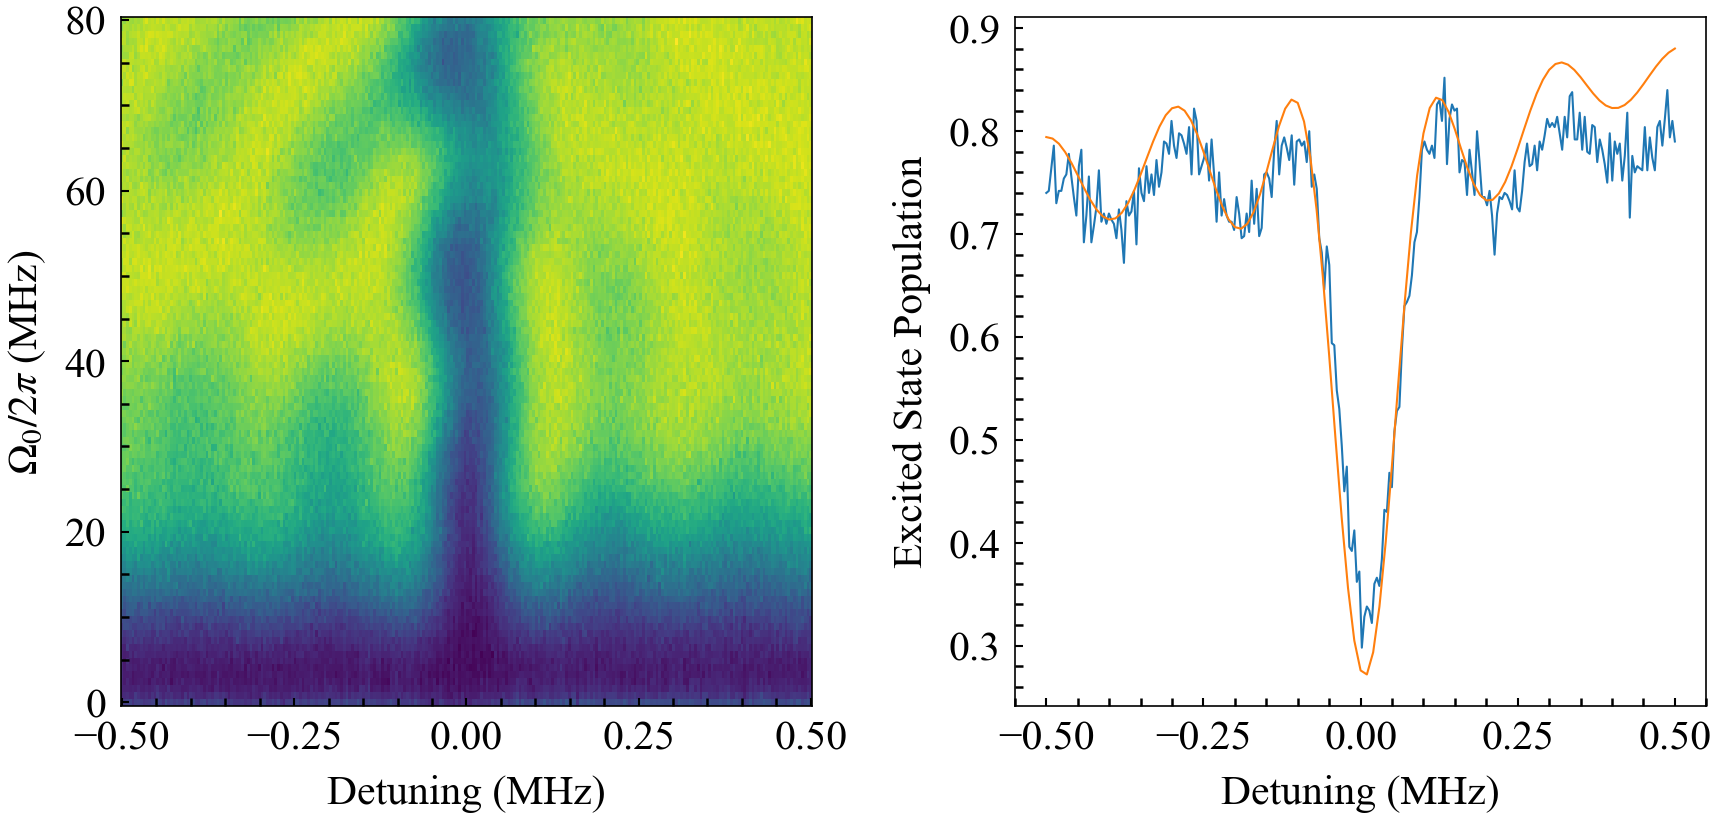
\includegraphics[width=1\linewidth]{figures/comparison.png}
    \caption{Two-dimensional spectroscopy map obtained with a 10 µs echo–root-Lorentzian pulse at extended drive amplitudes (up to 80 MHz). At shorter effective pulse durations and lower Rabi rates, distortions of the resonance profile become visible due to the proximity of the first two-photon transition. The left panel shows the full detuning–amplitude map, while the right panel presents a line cut at fixed drive strength (blue) together with a smooth fit (orange), highlighting deviations from an ideal single-photon response.}
    \label{fig:placeholder}
\end{figure}





